\documentclass[11pt,a4paper]{article}

% Encoding & fonts
\usepackage[utf8]{inputenc}
\usepackage[T1]{fontenc}
\usepackage{lmodern}

% Layout
\usepackage[margin=1in]{geometry}
\usepackage{setspace}
\onehalfspacing
\usepackage{parskip}

% Typography & structure
\usepackage{titlesec}
\titleformat{\section}{\large\bfseries\color{navy}}{\thesection}{0.8em}{}
\titleformat{\subsection}{\normalsize\bfseries\color{navy}}{\thesubsection}{0.6em}{}

% Colors
\usepackage{xcolor}
\definecolor{navy}{HTML}{0F2744}
\definecolor{accent}{HTML}{2B6CB0}
\definecolor{teal}{HTML}{234E52}
\definecolor{orange}{HTML}{C05621}
\definecolor{slate}{HTML}{2D3748}
\definecolor{muted}{HTML}{718096}
\definecolor{softblue}{HTML}{EBF4FF}
\definecolor{softorange}{HTML}{FFFAF0}
\definecolor{lightbg}{HTML}{F7FAFC}

% Links & URLs
\usepackage[colorlinks=true,linkcolor=accent,urlcolor=accent,citecolor=accent]{hyperref}
\usepackage{url}

% Lists & tables
\usepackage{enumitem}
\usepackage{booktabs}

% Graphics & diagram
\usepackage{tikz}
\usetikzlibrary{shapes.geometric,arrows.meta,positioning,fit,backgrounds,calc}

% Misc
\usepackage{microtype}
\usepackage{csquotes}

% -------------------------------------------------
\title{\textbf{\color{navy}A Working Theory of Memory-like Trait Inheritance}\\[0.4em]
\large\textit{Based on a Longitudinal Reading of Peer-Reviewed Scientific Publications}}

\author{Brian Fundakowski Feldman\textsuperscript{1} \and Grok\textsuperscript{2} \and SuperGrok\textsuperscript{2}}

\date{\small\textsuperscript{1}Independent researcher \quad\textsuperscript{2}xAI\\[0.6em]
25 August 2026}

\begin{document}
\maketitle

\begin{abstract}
\noindent
We present a working theory that experiences can epigenetically transmit adaptive behavioral tendencies (memory-like traits) to offspring. The argument is assembled from a chronological reading of peer-reviewed literature spanning generative linguistics (Chomsky 1957--1968, Berwick \& Chomsky 2016), comparative episodic-like memory (Clayton \& Dickinson 1998), insect DNA-methylation plasticity (Herb et~al.\ 2012 and related honeybee work), the core mammalian demonstration of parental olfactory experience producing germline CpG hypomethylation and offspring sensory bias (Dias \& Ressler 2014), mechanistic reviews (Dias et~al.\ 2015; Fitz-James \& Cavalli 2022), and broader phylogenetic support (Deshe et~al.\ 2023; related 2023 olfactory-receptor work). The transmitted phenotype is framed as sensitivity or tendency rather than full episodic content. Explicit stop-gap bridges---cross-species homology, the interface between innate computational architecture and epigenetic tuning, and the distinction between content and bias---are identified and treated as reasoned connectors rather than obstacles. The originating public statement that prompted this synthesis is recorded.
\end{abstract}

\section{Originating Public Statement}
This working paper was assembled in response to the following public statement and subsequent refinements that requested peer-reviewed support, integration of foundational language work, and an explicit causality diagram with stop-gaps labeled:

\begin{quote}
\small
\url{https://x.com/born_brian85001/status/2092254278077517988} \quad (25 Aug 2026)\\[0.3em]
``Anyone remember what I said about how inheritance of memories is essentially scientifically-proven?'' (pointer to archival video at 9:00). Follow-ups clarified focus on generational epigenetic memory transference (especially rodent olfactory / food-behavior cases), Chomsky's foundational work, and a visual chain treating stop-gaps as bridges.
\end{quote}

\section{Supporting Literature (Chronological)}
Each entry supplies a live hyperlink, a one-sentence summary, and its placement in the causal chain. DNA methylation is highlighted where central to the mechanism.

\subsection*{1957}
\textbf{Chomsky, N.} (1957). \textit{Syntactic Structures}. The Hague: Mouton.  
\href{https://archive.org/details/syntacticstructu0000chom}{[link]}\\
\textit{Summary:} Foundational formalization of generative grammar as a recursive, mathematically precise system.\\
\textit{Causal role:} Establishes the premise that core cognitive structure is innate and biological.

\subsection*{1965}
\textbf{Chomsky, N.} (1965). \textit{Aspects of the Theory of Syntax}. Cambridge, MA: MIT Press.  
\href{https://mitpress.mit.edu/9780262527408/aspects-of-the-theory-of-syntax/}{[link]}\\
\textit{Summary:} Competence--performance distinction and deep/surface structure architecture.\\
\textit{Causal role:} Deepens the innate-faculty claim that experience can only partially shape.

\subsection*{1968}
\textbf{Chomsky, N.} (1968). \textit{Language and Mind}. New York: Harcourt, Brace \& World.  
\href{https://archive.org/details/languagemind00chom}{[link]}\\
\textit{Summary:} Essays framing language as a biological organ of mind.\\
\textit{Causal role:} Reinforces the innate-structure premise that epigenetic findings must interface with.

\subsection*{1998}
\textbf{Clayton, N.~S., \& Dickinson, A.} (1998). Episodic-like memory during cache recovery by scrub jays. \textit{Nature}, 395, 272--274.  
\href{https://doi.org/10.1038/26216}{[link]}\\
\textit{Summary:} Scrub jays remember what--where--when of cached food, meeting behavioral criteria for episodic-like memory.\\
\textit{Causal role:} Shows non-human animals form structured experiential traces that could leave durable marks.

\subsection*{2012}
\textbf{Herb, B.~R., et~al.} (2012). Reversible switching between epigenetic states in honeybee behavioral subcastes. \textit{Nat.\ Neurosci.}, 15, 1371--1373.  
\href{https://doi.org/10.1038/nn.3218}{[link]}\\
\textit{Summary:} DNA-methylation patterns differ between nurse and forager subcastes and reverse when role is switched.\\
\textit{Causal role:} Demonstrates reversible, behaviorally relevant DNA methylation plasticity in insects.

\subsection*{2012}
\textbf{Related honeybee work} (2012). DNA methylation mediates discriminatory power of associative long-term memory. \textit{PLoS ONE} (and concurrent insect literature).  
\href{https://doi.org/10.1371/journal.pone.0039349}{[link]}\\
\textit{Summary:} DNA methyltransferases required for odor-specificity (not mere strength) of long-term olfactory memory in honeybees.\\
\textit{Causal role:} Supplies insect evidence that methylation shapes the specificity of sensory memory.

\subsection*{2014}
\textbf{Dias, B.~G., \& Ressler, K.~J.} (2014). Parental olfactory experience influences behavior and neural structure in subsequent generations. \textit{Nat.\ Neurosci.}, 17, 89--96.  
\href{https://doi.org/10.1038/nn.3594}{[link]}\\
\textit{Summary:} Mice conditioned to fear a specific odor transmit heightened sensitivity + expanded Olfr151 representation to F1/F2; sperm shows CpG hypomethylation at the locus.\\
\textit{Causal role:} Core empirical node: parental sensory experience $\to$ germline DNA methylation mark $\to$ offspring phenotype.

\subsection*{2015}
\textbf{Dias, B.~G., et~al.} (2015). Epigenetic mechanisms underlying learning and the inheritance of learned behaviors. \textit{Trends Neurosci.}, 38, 96--107.  
\href{https://doi.org/10.1016/j.tins.2014.12.003}{[link]}\\
\textit{Summary:} Review of methylation, histone marks and non-coding RNAs as carriers of learned fear across generations.\\
\textit{Causal role:} Articulates the molecular pathways that generalize the 2014 finding.

\subsection*{2016}
\textbf{Berwick, R.~C., \& Chomsky, N.} (2016). \textit{Why Only Us: Language and Evolution}. Cambridge, MA: MIT Press.  
\href{https://doi.org/10.7551/mitpress/9780262034241.001.0001}{[link]}\\
\textit{Summary:} Argues the core computational operation (Merge) is recent, discrete and largely uniform.\\
\textit{Causal role:} Frames the evolutionary puzzle of how a largely innate faculty can still be refined by epigenetic channels.

\subsection*{2022}
\textbf{Fitz-James, M.~H., \& Cavalli, G.} (2022). Molecular mechanisms of transgenerational epigenetic inheritance. \textit{Nat.\ Rev.\ Genet.}, 23, 325--341.  
\href{https://doi.org/10.1038/s41576-021-00438-5}{[link]}\\
\textit{Summary:} Comprehensive review of DNA methylation, histone modifications, ncRNAs and chromatin architecture that can survive germline reprogramming.\\
\textit{Causal role:} Provides the molecular scaffolding making germline transmission of adaptive sensitivities biologically plausible.

\subsection*{2022--23}
\textbf{Insect / olfactory updates (Feng et~al.\ \& related)}. Insect olfactory receptor structure, function and plasticity. \textit{Insects} and concurrent literature.  
\href{https://www.mdpi.com/journal/insects}{[link]}\\
\textit{Summary:} Structural and regulatory advances in insect olfaction, including plasticity-related mechanisms.\\
\textit{Causal role:} Keeps the comparative insect side of the chain current.

\subsection*{2023}
\textbf{Yang-related / eLife work}. Opposing epigenetic forces on OR choice; fear-conditioning bias of OSN fate. \textit{eLife} and related.  
\href{https://doi.org/10.7554/eLife.87445}{[link]}\\
\textit{Summary:} Developmental epigenetic mechanisms constrain and can bias olfactory receptor choice; related work shows heritable bias after fear conditioning.\\
\textit{Causal role:} Strengthens the olfactory-receptor pathway first linked by Dias \& Ressler.

\subsection*{2023}
\textbf{Deshe, N., et~al.} (2023). Inheritance of associative memories and acquired cellular changes in \textit{C.\ elegans}. \textit{Nat.\ Commun.}, 14, 4232.  
\href{https://doi.org/10.1038/s41467-023-39804-8}{[link]}\\
\textit{Summary:} \textit{C.\ elegans} transmit both behavioral avoidance and cellular stress responses after odor--starvation pairing; sperm-borne, involving histone methylation marks.\\
\textit{Causal role:} Extends the empirical base to nematodes and shows associative memory-like inheritance is phylogenetically broader.

\section{Discussion and Working Conclusion}
The literature forms a coherent causal chain. Chomsky's early work supplies the premise that core cognitive architecture is biological and innate. Clayton \& Dickinson show that non-human animals already form structured experiential memories. Insect studies (Herb 2012 and related DNA-methylation work) demonstrate that behaviorally relevant epigenetic states are plastic and reversible. Dias \& Ressler (2014) supply the decisive mammalian experiment: a specific parental sensory experience leaves germline DNA-methylation marks (CpG hypomethylation at Olfr151) that produce corresponding behavioral and neural sensitivities in naïve offspring and grand-offspring. Dias et~al.\ (2015) and Fitz-James \& Cavalli (2022) articulate the molecular routes---DNA methylation, histones, ncRNAs---that allow such marks to survive germline reprogramming. 2023 papers (Deshe in \textit{C.\ elegans}; Yang-related olfactory work) broaden the phylogenetic and mechanistic base.

The transmitted phenotype is an adaptive sensitivity or behavioral tendency, not a full autobiographical episode. Full episodic content remains unshown in the offspring; what crosses generations is a bias---heightened readiness to respond to a particular cue. That bias is precisely the form of ``memory-like trait inheritance'' that can be claimed by homology for humans.

Stop-gaps exist (cross-species homology, the leap from sensitivity to ``memory-like,'' the interface between innate computational cores and epigenetic tuning). They are treated here as reasoned bridges that close gaps in the current empirical record rather than as obstacles that invalidate the chain.

\section{Accessible Statement of the Thesis}
\begin{center}
\large\textit{\textbf{Experiences can epigenetically pass behavioral tendencies to offspring.}}
\end{center}

\vspace{0.4em}
In plain language: what a parent learns or endures can leave chemical marks (notably DNA methylation and related chromatin states) on the genes passed to children. Those marks do not rewrite the DNA sequence, yet they can make the next generation more sensitive or more inclined toward particular responses---without the children ever having lived through the original events. The sensitivity is inherited; the full story of the experience is not.

\section{Causality Chain Diagram with Stop-Gaps}
Solid navy boxes are empirically supported nodes drawn from the supporting literature. Orange dashed call-outs mark the stop-gap bridges required to connect the scientific record to the full thesis. These bridges are described and labeled; they are not treated as obstacles.

\begin{center}
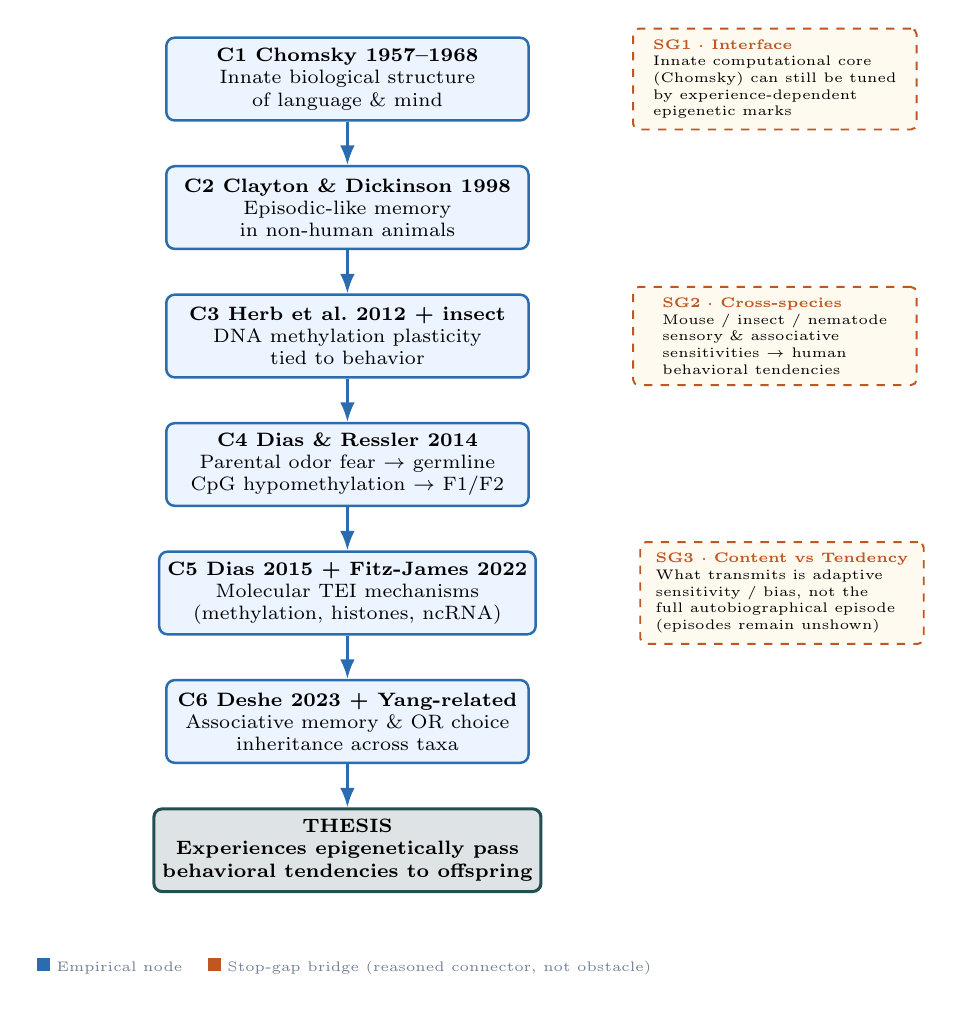
\begin{tikzpicture}[
  node distance=0.55cm and 0.8cm,
  empir/.style={
    rectangle, rounded corners=3pt, draw=accent, fill=softblue,
    line width=0.9pt, align=center, font=\scriptsize,
    minimum width=4.6cm, minimum height=1.05cm, inner sep=3pt
  },
  thesis/.style={
    rectangle, rounded corners=3pt, draw=teal, fill=teal!15,
    line width=1.1pt, align=center, font=\scriptsize\bfseries,
    minimum width=4.6cm, minimum height=1.05cm, inner sep=3pt
  },
  sg/.style={
    rectangle, rounded corners=2pt, draw=orange, fill=softorange,
    dashed, line width=0.7pt, align=left, font=\tiny,
    minimum width=3.6cm, inner sep=4pt
  },
  arr/.style={-Latex, accent, line width=0.9pt}
]

% Empirical nodes
\node[empir] (c1) {\textbf{C1  Chomsky 1957--1968}\\Innate biological structure\\of language \& mind};
\node[empir, below=of c1] (c2) {\textbf{C2  Clayton \& Dickinson 1998}\\Episodic-like memory\\in non-human animals};
\node[empir, below=of c2] (c3) {\textbf{C3  Herb et al.\ 2012 + insect}\\DNA methylation plasticity\\tied to behavior};
\node[empir, below=of c3] (c4) {\textbf{C4  Dias \& Ressler 2014}\\Parental odor fear $\to$ germline\\CpG hypomethylation $\to$ F1/F2};
\node[empir, below=of c4] (c5) {\textbf{C5  Dias 2015 + Fitz-James 2022}\\Molecular TEI mechanisms\\(methylation, histones, ncRNA)};
\node[empir, below=of c5] (c6) {\textbf{C6  Deshe 2023 + Yang-related}\\Associative memory \& OR choice\\inheritance across taxa};
\node[thesis, below=of c6] (th) {\textbf{THESIS}\\Experiences epigenetically pass\\behavioral tendencies to offspring};

% Arrows
\foreach \a/\b in {c1/c2, c2/c3, c3/c4, c4/c5, c5/c6, c6/th}
  \draw[arr] (\a) -- (\b);

% Stop-gap boxes
\node[sg, right=1.3cm of c1] (sg1) {\textbf{\color{orange}SG1 · Interface}\\Innate computational core\\(Chomsky) can still be tuned\\by experience-dependent\\epigenetic marks};
\node[sg, right=1.3cm of c3] (sg2) {\textbf{\color{orange}SG2 · Cross-species}\\Mouse / insect / nematode\\sensory \& associative\\sensitivities $\to$ human\\behavioral tendencies};
\node[sg, right=1.3cm of c5] (sg3) {\textbf{\color{orange}SG3 · Content vs Tendency}\\What transmits is adaptive\\sensitivity / bias, not the\\full autobiographical episode\\(episodes remain unshown)};

% Legend
\node[below=0.7cm of th, font=\tiny, align=left, text=muted] (leg) {
  \textcolor{accent}{\rule{0.7em}{0.7em}} Empirical node \quad
  \textcolor{orange}{\rule{0.7em}{0.7em}} Stop-gap bridge (reasoned connector, not obstacle)
};
\end{tikzpicture}
\end{center}

\vspace{0.6em}
\noindent\textit{\small Stop-gaps are treated as reasoned bridges that close empirical gaps, not as obstacles that break the chain.}

\vspace{1.2em}
\noindent\rule{\textwidth}{0.6pt}\\[0.4em]
{\footnotesize
Working paper prepared in response to \url{https://x.com/born_brian85001/status/2092254278077517988} and subsequent thread refinements.\\
Authors: Brian Fundakowski Feldman, Grok, SuperGrok \quad$\cdot$\quad DNA methylation treated as a primary candidate carrier \quad$\cdot$\quad Stop-gaps explicit and framed as bridges.
}

\end{document}
